\documentclass[11pt]{article}

\usepackage[review]{acl}

\usepackage{times}
\usepackage{latexsym}
\usepackage[T1]{fontenc}
\usepackage[utf8]{inputenc}
\usepackage{microtype}
\usepackage{inconsolata}
\usepackage{graphicx}
\usepackage{booktabs}
\usepackage{enumitem}
\usepackage{xcolor}
\usepackage{colortbl}

\definecolor{realblue}{HTML}{0072B2}
\definecolor{wrongred}{HTML}{D55E00}

\newcommand{\papertitle}{Worse Than Silence: Auditing KV-Cache Relay Between LLM Agents}
\title{\papertitle}

\author{Anonymous ACL submission}

\begin{document}
\maketitle

\begin{abstract}
Multi-agent LLM systems increasingly relay key-value (KV) caches instead of text, assuming the receiver reads what the cache says. Substituting a corrupted cache shows whether content matters, but not whether a wrong cache misleads the receiver or is ignored; that needs a receiver with no cache. We add this dropped condition to real, zeroed, random and mismatched caches and audit relay in a chain, a fan-in and model-driven delegation on Qwen2.5-7B, Mistral-7B and Qwen3-8B. A wrong cache is worse than none: another question's cache costs 30 accuracy points below no cache on Qwen2.5-7B and 23 on Mistral-7B (both Holm-significant). Wrong text also hurts, by 12 points, so the harm is generic and the cache amplifies it. Whether the real cache helps depends on whether it is the receiver's sole route to the evidence: hiding the passages from a chain's receivers turns the real cache from no better than none (56\% vs. 59\%) into far better (52\% vs. 20\%), and giving a fan-in aggregator the passages erases its benefit (55\% vs. 57\%). The gap survives int8 and KIVI-style int4 compression; Qwen3-8B shows no accuracy sensitivity. A wrong cache can be worse than silence.
\end{abstract}

\section{Introduction}

Multi-agent LLM pipelines increasingly pass each other the key--value (KV)
cache instead of decoded text, so that a receiving agent need not re-encode what
its sender already read \citep{kvcomm2025,latentmas2026}. The bet is that the
receiver reads what the cache says. But a KV cache is also just a tensor of the
right shape, and end-task accuracy cannot tell whether the receiver uses
its content, benefits from its mere presence, or would do as well without it.

Causal audits make this testable. \citet{latentcommpay2026} swap the
relayed cache for a zeroed, a moment-matched random, or a mismatched cache (another
question's real cache) and check whether accuracy follows the content. These
substitutes all still relay \emph{something}. \citet{zhangemu2026} add a no-message
baseline and measure an ``other-message effect'' against it, on Qwen3-4B and 8B with
GSM8K, ARC-Challenge and MATH-500, and find mixed signs: harmful on one model size,
helpful on another. Despite these efforts, it remains unclear how these
effects behave for KV relay on multi-hop QA, across model families, and across relay
topologies: does the real cache beat having none, and is a wrong cache merely
useless or actively harmful? Both matter in practice: a relay the receiver does not
need adds cost without benefit, and a relay that hurts when wrong turns a routing
error into lost accuracy.

\begin{figure}[t]
\centering
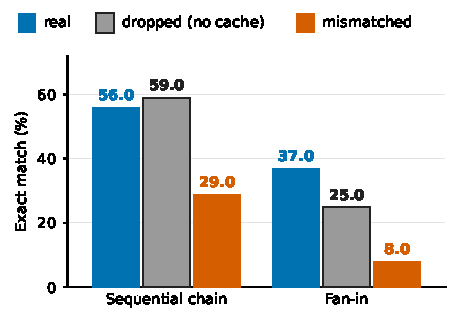
\includegraphics[width=\columnwidth]{figures/fig_headline.pdf}
\caption{Accuracy of Qwen2.5-7B on HotpotQA ($n{=}100$). A wrong cache is far worse than no
cache in both topologies. \textbf{Takeaway: a wrong cache is worse than no cache; the
real cache is not clearly better than none in the chain.}}
\label{fig:headline}
\end{figure}

\begin{figure*}[t]
\centering
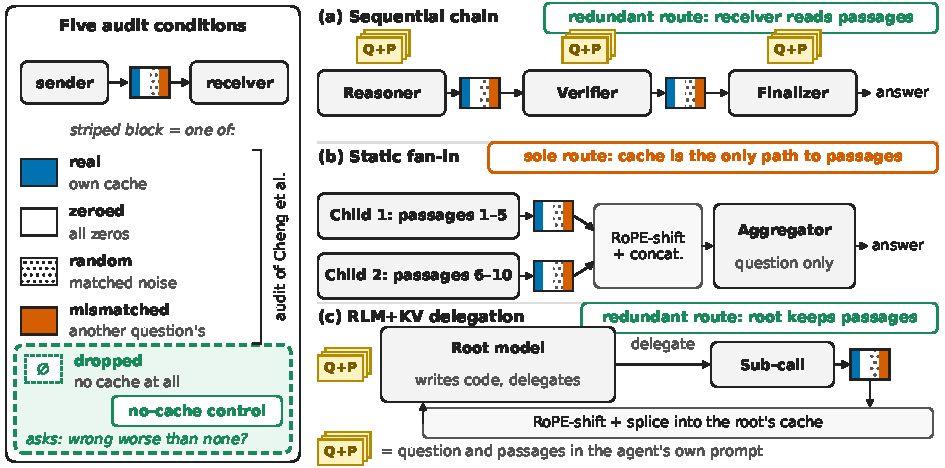
\includegraphics[width=\textwidth]{figures/fig1_overview.pdf}
\caption{The five-condition causal audit (left) and the three relay
topologies (right). At each audit point (striped block) the relayed KV cache is
replaced by one of five conditions; the first four follow
\citet{latentcommpay2026}, and dropped follows the no-message baseline of
\citet{zhangemu2026}. (a) Chain: receivers also read the passages (Q+P), so the
cache is redundant. (b) Fan-in: the aggregator sees only the question and the
merged caches, so the cache is its sole route. (c) RLM+KV: a root model delegates
through code and splices sub-call caches into its own while keeping the passages.
\textbf{Takeaway: by varying the relayed cache, and whether it is the receiver's
only route to the evidence, the audit separates a cache the receiver needs from one
that merely hurts when wrong.}}
\label{fig:overview}
\end{figure*}

To address this, we study KV relay with a five-condition audit at the point
of relay (Figure~\ref{fig:overview}): real, zeroed, random, mismatched, and
\emph{dropped}, in which the receiver keeps its unchanged prompt and receives no
cache. The dropped condition follows the no-message baseline of
\citet{zhangemu2026}; we apply it to three relay topologies, a second model family,
multi-hop QA and compressed relays. Our goal poses two challenges: (1)
telling a cache the receiver needs apart from one that merely hurts when wrong, and
(2) telling whether the answer depends on how the receiver gets the
evidence. For (1), we compare real, mismatched and dropped caches. For (2), we
choose topologies that differ in whether the cache is the receiver's only route to
the evidence. In a three-agent chain (Reasoner, Verifier, Finalizer), each receiver
also reads the passages, so the cache is redundant. In a static fan-in, two children
each read five of the ten passages and the aggregator sees only the question and
their merged cache, so the cache is its sole route. In RLM+KV, a root model in the
style of Recursive Language Models \citep{rlm2026} decides through code what to
delegate and splices each sub-call's cache into its own, while keeping the passages.
We test Qwen2.5-7B-Instruct, Mistral-7B-Instruct-v0.3 and Qwen3-8B, mostly on
HotpotQA \citep{hotpotqa2018} ($n{=}50$--$100$ per condition; exact McNemar tests;
Holm correction over a designated primary family).

The no-cache baseline changes what the audit can say (Figure~\ref{fig:dotplot}).
A wrong cache is worse than none: no cache beats mismatched 59.0\% vs.\
29.0\% on Qwen2.5 and 49.0\% vs.\ 26.0\% on Mistral in the chain ($n{=}100$;
$p<0.0001$ and $p=2\times10^{-4}$), and 25.0\% vs.\ 8.0\% in the fan-in
($p=7.6\times10^{-5}$); all survive Holm correction (Figure~\ref{fig:headline}). Whether the real cache
matters depends on passage access. With the passages in the receivers' prompts,
real is not shown to beat no cache ($p=0.68$, $0.45$, $1.0$ on the three models).
Hiding the passages from the chain's receivers drops no cache from 59.0\% to 20.0\%
while real barely moves (56.0\% to 52.0\%), so real beats no cache by 32 points
($p<10^{-6}$); giving the fan-in aggregator the passages does the converse, erasing
real's edge (55.0\% vs.\ 57.0\%, $p=0.80$). The harm is not KV-specific, but
the cache amplifies it: wrong text costs 12 points (59.0\% to 47.0\%,
$p=0.0005$) against 30 for the cache (gap 18 points, 95\% CI $[7,29]$). Text relay
also shows the sole-route pattern and ties the cache in the passage-hidden chain
(48.0\% vs.\ 52.0\%, $p=0.45$), but beats the fan-in's merged cache (51.0\% vs.\
37.0\%, $p=0.009$). Qwen3-8B, run in non-thinking mode, is the exception: accuracy
is insensitive to cache content, and mismatched and dropped outputs are identical
on 80 of 100 examples.

\begin{figure}[!t]
\centering
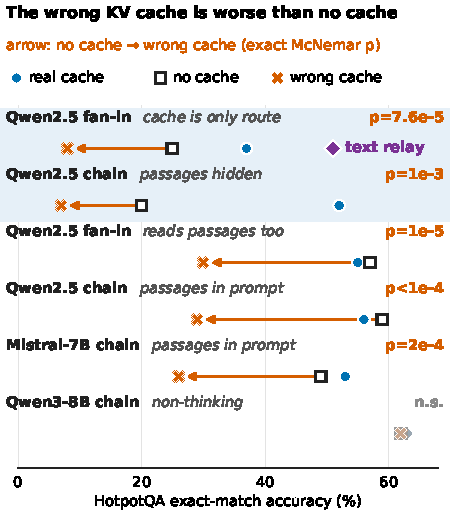
\includegraphics[width=\columnwidth]{figures/fig2_dotplot.pdf}
\caption{Exact-match accuracy when the receiving agent gets its real relayed KV
cache ($\bullet$), no cache (open square), or the real cache of a different question
($\times$); $n{=}100$ in every row. Arrows show the drop from no cache to the
wrong cache (exact McNemar $p$). In the fan-in (shaded) the cache is the
aggregator's only route to the passages: real far exceeds wrong, yet text relay
($\diamond$) exceeds real. The shaded chain row hides the passages from the
receivers, which makes real far exceed no cache; in the unshaded rows, including
the fan-in whose aggregator also reads the passages, the receiver has its own copy
and real is not distinguishable from no cache. Qwen3-8B (non-thinking mode, grey) shows
no detectable accuracy sensitivity.
\textbf{Takeaway: on Qwen2.5 and Mistral, replacing no cache with the wrong cache
costs 23 to 30 accuracy points in the chain; a wrong cache is worse than none.}}
\label{fig:dotplot}
\end{figure}

The same audit doubles as a test of compression. An int8 relay
(2.00$\times$) and a KIVI-style per-channel int4 relay \citep{kivi2024}
(3.96$\times$) keep the real-versus-mismatched gap on Qwen2.5 and Mistral, so
compression does not turn the cache into generic state. Naive int4 collapses to
0.0\%, which we attribute to keys being cached after RoPE has been applied
(Appendix~\ref{app:rotation}).

We do not claim that KV relay improves accuracy or latency. In the fan-in
text relay beats it, and in the chain text relay (54.0\%), a single agent (57.0\%)
and KV relay (56.0\%) score similarly (Appendix Table~\ref{tab:full}). Our
evaluation is single-GPU, uses $n{=}50$--$100$ per condition, and is mostly
HotpotQA. Our contributions are:

\begin{itemize}[leftmargin=*,itemsep=2pt,topsep=2pt]
\item \textbf{The no-cache comparison, applied to KV relay across topologies.}
Following \citet{zhangemu2026}, we show on multi-hop QA that wrong content is
actively harmful on Qwen2.5 and Mistral: replacing no cache with a mismatched
cache costs 30 accuracy points on Qwen2.5 and 23 on Mistral (both
Holm-significant), in contrast to the mixed signs reported on Qwen3 math and
science tasks. A text-relay control shows the harm is generic (wrong text costs 12
points) but amplified by the cache (30 points).
\item \textbf{Sole and redundant routes, compared rather than averaged.} Auditing
a sole-route fan-in next to redundant-route chains (and a delegation loop) helps
explain why relay results need not transfer between systems: real beats
mismatched 37.0\% vs.\ 8.0\% in the fan-in, while in the chain real is not shown
to beat no cache. Controlled ablations in both directions support the account:
hiding the passages from the chain's receivers raises real over no cache from $-3$
to $+32$ points, and giving the fan-in aggregator the passages lowers it from $+12$
to $-2$.
\item \textbf{A practical negative result.} In the fan-in, text relay beats the
merged KV cache by 14 accuracy points (51.0\% vs.\ 37.0\%), yet the two tie in the
passage-hidden chain (48.0\% vs.\ 52.0\%): the deficit is tied to merging
independently computed caches, not to the KV channel itself. A KV channel should
still be justified against a text baseline, not only against noise.
\item \textbf{Compression under the audit.} Accuracy alone cannot show that a
compressed relay still carries content; the audit can. KIVI-style int4 keeps the
real-versus-mismatched gap at 3.96$\times$.
\item \textbf{A reported exception.} Qwen3-8B in non-thinking mode shows no
detectable accuracy sensitivity to cache content, so content dependence should be
audited per model rather than assumed.
\end{itemize}

\section{Related Work}
\label{sec:related}

\paragraph{Relaying state instead of text.} KVCOMM \citep{kvcomm2025}
corrects KV-cache offset drift when reusing cache across prefixes, and
LatentMAS \citep{latentmas2026} lets agents exchange latent ``thoughts''
through KV working memory; KVComm \citep{shikvcomm2025} is a distinct
system with a near-identical name. Recursive Language Models
\citep{rlm2026} let a root model delegate through a sandboxed REPL
rather than a fixed topology, and CanonicalMerge
\citep{canonicalmerge2026} studies merging parallel caches, reporting
downstream accuracy only. None of these tests whether the relayed
content is causally necessary.

\paragraph{Auditing whether relay carries content.}
\citet{latentcommpay2026} audit three published relay systems with zeroed,
moment-matched random and deranged (mismatched) substitution and find
content-specificity is system-dependent; their no-communication control is a
zeroed cache rather than an empty one. \citet{zhangemu2026} audit latent
channels, including KV caches, on Qwen3-4B/8B with GSM8K, ARC-Challenge and
MATH-500; they include a no-message baseline, define an other-message effect
against it, and report mixed signs that reverse between model sizes.
\citet{latentagentslie2026} audit cache integrity under an adversarial agent.
We adopt the substitution methodology and the no-message comparison, and apply
them in ways neither prior audit covers: three topologies, including one the
model constructs itself; a second model family and multi-hop QA, where the
other-message effect is strongly negative on two of three models; and
compressed relays. Our Qwen3-8B result parallels the system and model-size
dependence both papers report (Appendix~\ref{app:relwork}).

\paragraph{Why a wrong message can hurt.} That irrelevant or conflicting
context degrades LLM answers is well documented: models are distracted by
irrelevant context \citep{shi2023distracted}, use information unevenly across a
long context \citep{liu2024lost}, and respond to conflicting evidence in ways
that depend on how coherent it looks \citep{xie2024knowledgeconflicts}. A
mismatched cache is a form of this, delivered as hidden state rather than
text. Whether the harm is specific to the KV channel or generic to any wrong
inter-agent message is what a text-relay control answers; we run one
(Section~\ref{sec:results}) and find the harm is generic but larger for the cache.

\paragraph{KV compression and layer selection.} Quantization and layer
dropping shrink the relayed cache. KIVI \citep{kivi2024}, RotateKV
\citep{rotatekv2025} and KVQuant \citep{kvquant2024} identify the
difficulty of quantizing post-RoPE keys, which we confirm when a
rotation-based scheme in the style of TurboQuant \citep{turboquant2026}
and PolarQuant \citep{polarquant2026} fails on our pipeline
(Appendix~\ref{app:rotation}). ``No Free Swap'' \citep{nofreeswap2026}
finds layer redundancy depends on model and protocol, consistent with
our layer-selection results (Section~\ref{sec:results}). We use these
techniques only to test whether the causal finding survives compression;
further related work is in Appendix~\ref{app:relwork}.

\section{Audit Design}
\label{sec:method}

\paragraph{Conditions.} At the point a cache would be relayed we
substitute one of five contents (Table~\ref{tab:conditions}); we say ``wrong
cache'' for \emph{mismatched} and ``no cache'' for \emph{dropped}. Zeroed and
random are out-of-distribution sanity floors. Mismatched and dropped are the
informative pair: a mismatched cache is exactly as valid a tensor as the real
one, and dropped says whether wrong content is worse than having none. Donor caches come from a pool of 20 held-out
questions never among the scored set, with one donor draw per scored
example. In every condition the receiver's prompt is unchanged, so only
the cache varies; this makes the prompt's statement that prior content is
in context literally false under dropped, a choice that works against,
not for, our finding that wrong is worse than none.

\begin{table}[t]
\centering
\small
\caption{What the receiver's cache holds under each condition.}
\label{tab:conditions}
\begin{tabular}{lp{5.2cm}}
\toprule
\textbf{Condition} & \textbf{Cache the receiver attends over} \\
\midrule
real       & the sender's own cache \\
dropped    & none: the receiver's own prompt only \\
zeroed     & all-zero tensors, same shape \\
random     & noise matching each tensor's mean and std \\
mismatched & a real cache from a different held-out question \\
\bottomrule
\end{tabular}
\end{table}

\paragraph{Topologies (Figure~\ref{fig:overview}).} The sequential chain is a three-agent
pipeline (Reasoner, Verifier, Finalizer) in which each downstream agent's
prompt already contains the source passages. In the fan-in, the
ten HotpotQA passages are split across two child agents; their
RoPE-shifted caches are concatenated, and the aggregator sees only the
question plus the merged cache, with no independent copy of the passages.
In the model-driven delegation loop (RLM+KV), a root model writes
code in a sandboxed REPL and decides what to delegate; a sub-call's cache
is RoPE-shifted and spliced onto the root's, and the root keeps direct
access to the passages. No agent framework exposes KV cache as a
channel, so all three are built directly on \texttt{transformers}
\citep{transformers2020} (Appendix~\ref{app:method-ext}).

\paragraph{Implementation.} Every configuration shares the same
Reasoner, Verifier and Finalizer prompts as a text-relay baseline that
passes decoded text instead of cache, so differences between relay
variants are attributable to the relayed content, not to prompt wording.
All decode paths use the same repetition penalty (1.05) and the
\texttt{sdpa} attention backend. Quantized and layer-selected variants
(8-bit and 4-bit per-head or per-channel min--max quantization; dropping
calibration-identified low-importance layers with zero reconstruction) are
audited with the same five conditions.

\paragraph{Models and data.} Qwen2.5-7B-Instruct \citep{qwen2p5_2024} is
the primary model in all three topologies. Mistral-7B-Instruct-v0.3
\citep{mistral7b2023} and Qwen3-8B \citep{qwen3_2025} (non-thinking mode)
run the chain only. We use HotpotQA (distractor setting) with a GSM8K
\citep{gsm8k2021} and a 2WikiMultihopQA replication in
Appendix~\ref{app:results-ext}. All runs use bf16, greedy decoding and one
RTX 4090.

\paragraph{Statistics.} We report accuracy (exact match) and token F1,
exact paired McNemar tests on per-example correctness, and paired
bootstrap 95\% CIs (10{,}000 resamples) on F1 differences. We designate
eight primary comparisons (real vs.\ mismatched and dropped vs.\
mismatched, per model and topology) and Holm-adjust them
(Appendix~\ref{app:stats}); the family was fixed after the initial
$n{=}50$ runs, and the Qwen2.5 and Mistral chains and the Qwen2.5 fan-in were
then re-run at $n{=}100$, which we disclose as a form of optional stopping. The
passage-access ablations and donor-seed runs had expected outcomes stated in
advance, not formally preregistered; the text-relay comparison was exploratory. Every
other $p$-value is descriptive and uncorrected.

\section{Results}
\label{sec:results}

\subsection{Sequential chain: wrong is worse than none}

\paragraph{Content matters at all.} On the uncompressed chain
(config \texttt{A}, Qwen2.5, $n{=}50$), real scores 50.0/64.0
(accuracy/F1) against 0.0/0.0 for zeroed and random and 28.0/37.1 for
mismatched; real beats zeroed and random at $p<0.0001$ and mismatched at
$p=0.0127$ (Appendix Table~\ref{tab:ladder}). The same ordering holds for the
compressed and layer-selected configurations (Appendix
Table~\ref{tab:causal_audit_full}) and replicates on a second task and
dataset: on GSM8K, real scores 90.0\% against 0.0\% zeroed, 2.0\% random and
28.0\% mismatched (all $p<0.0001$), and on 2WikiMultihopQA 54.0/62.5 against
0.0/0.7, 0.0/0.0 and 16.0/23.4 (real vs.\ mismatched $p=0.000004$, 19 of 19
discordant pairs favoring real).



\begin{table*}[t]
\centering
\small
\caption{Dropped (no-cache) control. Accuracy / F1 (\%) per condition; exact
paired McNemar $p$-values, uncorrected (Holm-adjusted values for the
primary family are in Appendix~\ref{app:stats}). All rows use
$n{=}100$. $^\dagger$Qwen3-8B ran with thinking disabled, so an
architecture effect cannot be separated from a decoding-mode effect.}
\label{tab:no_relay}
\begin{tabular}{lccccccc}
\toprule
 & \multicolumn{3}{c}{\textbf{Accuracy / F1}} & \multicolumn{3}{c}{\textbf{$p$-value}} & \\
\cmidrule(lr){2-4}\cmidrule(lr){5-7}
\textbf{Model / topology} & \textcolor{realblue}{\textbf{Real}} & \textbf{Dropped} & \textcolor{wrongred}{\textbf{Mismatched}} & Real\,/\,Dropped & Real\,/\,Mism. & Dropped\,/\,Mism. & $n$ \\
\midrule
Qwen2.5-7B, chain        & 56.0/69.1 & 59.0/69.0 & 29.0/40.6 & 0.68  & 0.000025 & $<$0.0001 & 100 \\
Mistral-7B, chain        & 53.0/65.1 & 49.0/59.7 & 26.0/36.5 & 0.45  & 0.0000014 & 0.0002   & 100 \\
Qwen3-8B, chain$^\dagger$& 63.0/75.3 & 62.0/72.8 & 62.0/71.6 & 1.0   & 1.0      & 1.0       & 100 \\
\midrule
Qwen2.5-7B, fan-in       & 37.0/46.6 & 25.0/33.4 & 8.0/13.0  & 0.050 & $<$0.0001 & 0.000076 & 100 \\
\bottomrule
\end{tabular}
\end{table*}

\paragraph{Wrong is worse than none.} Table~\ref{tab:no_relay} shows the
central result. On Qwen2.5 and Mistral, a mismatched cache is worse than
no cache ($p<0.0001$ and $p=0.0002$) and worse than the real cache
($p=0.000025$ and $p=0.0000014$): wrong content is not merely unhelpful,
it is actively harmful relative to having none. Manual review of 20 of the
36 wrong mismatched answers finds donor-question content leaking into the
output only rarely (one clear case; Appendix~\ref{app:results-ext}), so
the harm is mostly confusion on the real question rather than topic
substitution. The result does not hinge on which donors are drawn: three
independent donor draws on Qwen2.5 score 29.0\%, 23.0\% and 23.0\% mismatched (no
pair of draws differs significantly, $p\ge0.24$), and no cache (59.0\%) stays far
above all three (30 to 36 points; $p\le10^{-4}$ for each). Three Mistral draws
agree too (26.0\%, 19.0\% and 21.0\% mismatched, no pair significantly different,
$p\ge0.17$; 23 to 30 points below the 49.0\% for no cache).

\begin{table*}[t]
\centering
\small
\caption{Wrong text versus wrong cache (Qwen2.5-7B chain, $n{=}100$, same
questions). Accuracy / F1 (\%); exact paired McNemar $p$-values. Harm is no cache
minus mismatched, in accuracy points. Text relay passes the previous agent's
decoded answer; KV relay passes its cache. In the hidden rows the passages are
removed from the Verifier's and Finalizer's own prompts.}
\label{tab:textctrl}
\begin{tabular}{llccccccc}
\toprule
\textbf{Channel} & \textbf{Passages} & \textcolor{realblue}{\textbf{Real}} & \textbf{Dropped} & \textcolor{wrongred}{\textbf{Mismatched}} & $p$(Real, Dropped) & $p$(Dropped, Mism.) & \textbf{Harm} \\
\midrule
KV relay   & in prompt & 56.0/69.1 & 59.0/69.0 & 29.0/40.6 & 0.68 & $7\times10^{-8}$ & 30 \\
Text relay & in prompt & 54.0/68.3 & 59.0/68.9 & 47.0/57.8 & 0.36 & 0.0005           & 12 \\
\midrule
KV relay   & hidden    & 52.0/66.0 & 20.0/29.6 & 7.0/12.1  & $4\times10^{-7}$ & 0.001 & 13 \\
Text relay & hidden    & 48.0/59.2 & 20.0/30.0 & 14.0/18.6 & $4\times10^{-6}$ & 0.15  & 6 \\
\bottomrule
\end{tabular}
\end{table*}

\paragraph{Wrong text hurts too, but less.} To test whether the harm is specific
to the KV channel, we relay another question's decoded text in the same slot
(Table~\ref{tab:textctrl}). Wrong text is also worse than no relay (59.0\%
vs.\ 47.0\%, $p=0.0005$; 12 examples favor no relay and none favor wrong text), so
the harm is not specific to KV, in line with the distractor literature
\citep{shi2023distracted}. The cache amplifies it: wrong cache scores 29.0\%
against 47.0\% for wrong text on the same questions ($p=0.002$), and the harm gap of
18 points has a paired bootstrap 95\% CI of $[7,29]$ points. With correct content the
channels tie (54.0\% text vs.\ 56.0\% cache, $p=0.82$). With the passages
hidden, the picture is similar but weaker: text relay shows the same sole-route
benefit as the cache (48.0\% vs.\ 20.0\% for no relay, $p=4\times10^{-6}$; cache
52.0\% vs.\ 20.0\%), the two channels tie (52.0\% vs.\ 48.0\%, $p=0.45$), and wrong
text costs 6 points ($p=0.15$) against 13 for the wrong cache (gap 7 points, 95\% CI
$[0,15]$, $p=0.065$); no cache scores only 20.0\% there, so a floor effect limits
this comparison. One confound limits the reading: the wrong cache carries the donor's passages as well as its reasoning,
while wrong text carries only the reasoning, so the cache's larger harm may reflect
more misleading material rather than anything about hidden state itself.

\paragraph{Real is not distinguishable from no cache.} The real cache does
not beat dropped on any model in the chain: $p=0.68$ (Qwen2.5), $0.45$ (Mistral) and
$1.0$ (Qwen3-8B), with the point estimate pointing in different
directions across models. Doubling Qwen2.5's sample from $50$ to $100$
moved the estimate toward zero, not away from it (56.0\% vs.\ 59.0\%, F1
difference $+0.1$, 95\% CI $[-8.2,+8.4]$). We read this as
indistinguishable at this sample size, not as evidence that the cache is
unnecessary or that the two are equivalent. In line with this, a single
agent with no relay (57.0/68.4) and the full relay chain (56.0/69.1) score
similarly (Appendix Table~\ref{tab:full}); we ran no paired test between
them.

\paragraph{What we ruled out.} We checked the failure modes a skeptical
reader would raise:
\begin{itemize}[leftmargin=*,itemsep=1pt,topsep=2pt]
\item \emph{Donor leakage.} Every mismatched donor question was compared with
its scored question directly; none overlap.
\item \emph{Garbled output as a scoring artifact.} A garbage-signature scan
over fan-in generations flags 0/50 real, 4/50 mismatched, 23/50 zeroed and
48/50 random outputs, a monotone ordering that matches accuracy. Random noise
is more degraded than zeros: a zero key is weak and can be down-weighted,
while realistic noise resembles signal and misdirects attention.
\item \emph{Decoding confound.} Qwen's default repetition penalty is our
setting (1.05) and Mistral's specifies none, so our setting corrects
\emph{more} for Mistral, the opposite of what an unfair-to-Mistral confound
needs.
\item \emph{Reproducibility.} Greedy decoding is bit-identical across reruns
in the chain and fan-in, in the delegation loop after our determinism fix, and in
the text-relay control (all 300 raw answers and all 100 donor assignments match
between a resumed run and a fresh run).
\end{itemize}

\subsection{Fan-in: when the cache is the only route}

In the fan-in the picture changes. Dropped falls to 25.0/33.4, well below
real (37.0/46.6), because the aggregator has no other copy of the passages;
dropped here is effectively a closed-book run, so 25.0\% is what the aggregator
answers from parametric knowledge alone. Real versus dropped is borderline ($p=0.050$, F1 difference
$+13.2$, 95\% CI $[+2.2,+24.2]$, which excludes zero); at $n{=}50$ it was
$p=0.12$. Real decisively beats mismatched ($p<0.0001$, 30 of 31
discordant pairs), and dropped still beats mismatched ($p=0.000076$, 18
of 19 discordant pairs): even where the cache is the only route to the
evidence, a wrong one is worse than none. At $n{=}50$ the full ladder is
clean: real 40.0/53.0, zeroed 0.0/0.8, random 0.0/0.0, mismatched
6.0/12.0 (real vs.\ mismatched $p=0.0001$).

\paragraph{Text relay beats KV relay here.} The same fan-in with the children's
decoded answers passed as text, instead of their caches, scores 51.0/60.9 against
37.0/46.6 for the real cache ($n{=}100$, exact McNemar $p=0.009$; 20 examples
favor text and 6 favor KV; F1 difference $+14.4$, 95\% CI $[+5.0,+23.8]$). Text
relay also far exceeds no cache (51.0\% vs.\ 25.0\%, $p<0.0001$). Even where
the cache is the receiver's only route, it recovers under half (12 of 26 points) of
the gain that text relay provides over no relay. This gap is specific to
the fan-in's merge, not to the KV channel: when a single sequential cache is the
only route (the passage-hidden chain), cache and text tie (52.0\% vs.\ 48.0\%,
$p=0.45$). A plausible reason is that the two children's caches were computed in
isolation and never attend to each other, whereas text lets the aggregator read both
answers jointly; the chain tie is consistent with this, but we have not tested it
directly. The KV results are bit-identical across the two runs.



\paragraph{Passage access, tested in both directions.} To test whether passage
access, rather than topology, drives the difference, we intervene on it directly
(Appendix Table~\ref{tab:nopass}; the rows are plotted in
Figure~\ref{fig:dotplot}). In the chain, we remove the passages from the
Verifier's and Finalizer's own prompts, so the relayed cache is their only route.
Hiding the passages flips the result: no cache collapses from 59.0\% to
20.0\% ($p=2\times10^{-10}$), near the fan-in's closed-book 25.0\%, while the real
cache barely moves (56.0\% to 52.0\%, $p=0.39$), so it carries enough of the
passages' content to stand in for reading them. Real now beats no cache by 32
points ($p=4\times10^{-7}$; F1 difference $+36.5$, 95\% CI $[+25.6,+47.2]$), and
mismatched stays below no cache (7.0\% vs.\ 20.0\%, $p=0.001$). In the
fan-in, we do the converse and put all ten passages in the aggregator's prompt:
no cache rises from 25.0\% to 57.0\% ($p=7\times10^{-8}$), the real cache from
37.0\% to 55.0\% ($p=3\times10^{-4}$), and real's edge over no cache disappears
(55.0\% vs.\ 57.0\%, $p=0.80$; F1 difference $+0.2$, 95\% CI $[-5.9,+6.0]$), while
a mismatched cache still hurts (30.0\%, $p=1\times10^{-5}$ against no cache). So
giving the receiver another route removes the real cache's benefit but not
a wrong cache's harm. We stated both expected outcomes in advance, without formal preregistration. The
topologies still differ in other ways, so these are interventions on passage
access, not on topology as a whole.

\subsection{Model-driven delegation}

The RLM+KV loop is the least favorable topology for a clean result: our
HotpotQA questions do not need decomposition, and the root can read the
passages directly. Accuracy of \texttt{kv} against \texttt{text} relay is
unresolved at $n{=}50$ (24.0/32.3 vs.\ 22.0/28.5, $p=1.0$), and we claim
no KV accuracy win. The audit still resolves: \texttt{kv} beats zeroed
($p=0.0078$), random ($p=0.0039$) and mismatched ($p=0.0156$), with F1
differences of $+0.210$, $+0.230$ and $+0.167$ (all CIs exclude zero).
Zeroed and random land at 8.0\% and 6.0\% rather than near zero because
the root's direct path to the passages bypasses the audited channel, so
this audit is narrower than the other two. The dropped control here is
directionally consistent but not significant (\texttt{kv} vs.\ dropped
$p=0.22$; dropped vs.\ mismatched $p=0.25$, 3 of 3 discordant pairs favor
dropped). Whether a session finishes within its turn budget tracks the
same ordering and resolves the leg accuracy cannot: the share of sessions
that time out is 22\% for real, 42\% for mismatched, 72\% for zeroed and 76\%
for random, with every pairwise difference significant, including mismatched
vs.\ random ($p<0.0001$; Appendix~\ref{app:behavioral}). The prototype is
bit-identically reproducible under our determinism fix
(Appendix~\ref{app:nondeterminism}).

\subsection{Architecture dependence}

\paragraph{Qwen3-8B shows no detected accuracy sensitivity to cache content.}
At $n{=}100$, real, dropped and mismatched score 63.0\%, 62.0\% and 62.0\% (all
three pairwise $p=1.0$; F1 75.3, 72.8, 71.6), and mismatched and dropped give the
identical output string on 80 of 100 examples, so the model effectively
ignores a wrong cache. The real cache is not ignored: only 41 of 100 outputs match
those of dropped, yet with no net accuracy change. Random noise still collapses
accuracy ($p<0.0001$) and real is indistinguishable from zeroed
($p=0.30$--$0.79$ across four $n{=}50$ comparisons on configurations \texttt{A} and
\texttt{D}). We checked this is not a bug (no donor leakage, selective
substitution; Appendix~\ref{app:qwen3}).
It is consistent with robustness to irrelevant context but, because the
run used non-thinking mode, we cannot separate an architecture effect from
a decoding-mode effect.

The same model dependence appears in layer selection: dropping a near-identical
share of layers costs 30.5 F1 points on Mistral ($p=0.0001$) but a smaller,
not significant amount on Qwen2.5 ($p=0.34$) and nothing detectable on
Qwen3-8B (Appendix~\ref{app:results-ext}).

\subsection{Compression does not make the cache generic}

If the cache carried only generic state, compressing it should not matter; if
it is content-specific, compression should leave the real-versus-mismatched gap
intact. It does. \texttt{B\_int8} and \texttt{B\_int4\_kivi} keep the gap on
Qwen2.5 and Mistral (Appendix Table~\ref{tab:causal_audit_full}; on Qwen2.5, real vs.\ mismatched is
$p\le0.02$ for \texttt{B\_int8}, \texttt{B\_int4\_kivi} and the layer-selected
configurations \texttt{C} and \texttt{D}), as Appendix Figure~\ref{fig:compression} shows.
\texttt{B\_int8} is indistinguishable from uncompressed relay ($p=1.0$, 3
discordant of 100) at 2.00$\times$ smaller. Uniform 4-bit quantization
collapses to 0.0/0.0, which we attribute to keys being cached after RoPE;
quantizing keys per channel (KIVI-style) recovers 52.0/64.1 at 3.96$\times$
compression (Appendix Table~\ref{tab:main}). The 3.96$\times$ ratio comes from a
packing-enabled compressor applied after accuracy was measured on the unpacked
version (Appendix~\ref{app:nibble}). We report compressed bytes and make no
latency claim: nothing is transmitted over a network and every layer still runs.



\section{Discussion}

\paragraph{For system designers.} Audit a relay channel against silence,
not only against noise. In our setting a wrong cache scored below no cache on two
of three models, and wrong text did too, so provenance matters for any channel and
more for the cache. Where a cache's provenance cannot be guaranteed (for example
when caches are reused across contexts), dropping it may be the safer fallback,
though not a free one where the cache is the receiver's only route (the fan-in).
This is motivation for auditing, not a general recommendation: our wrong caches
are injected, and we have not measured how often real deployments misroute.

\paragraph{When the real cache matters.} The real cache clearly helps
only where it carries evidence the receiver cannot get elsewhere, as the
passage ablations show: the same chain goes from no benefit to a 32-point benefit
when its receivers lose their own copy of the passages, and the fan-in loses its
benefit when the aggregator gains one. The delegation loop, where
the root keeps its own path to the passages, shows the weakest effects, as this
account predicts.

\paragraph{KV relay against a text baseline.} A KV channel should be
justified against a text baseline, not only against noise. In our fan-in, text
relay beats the merged cache by 14 accuracy points, but in the passage-hidden chain
the two tie (48.0\% text vs.\ 52.0\% cache), and with the passages in the prompt
text relay, a single agent and KV relay score within three points of each other.
The fan-in deficit therefore reflects merging independent caches, not KV as a
channel. Latency is
not a clean test in our single-GPU setup, which transmits nothing over a network
(KV relay was not faster: 8.6 s vs.\ 7.2 s per example for text in the chain,
Appendix Table~\ref{tab:full}), so these results bound the accuracy case only.

\paragraph{Per-model audits.} Qwen3-8B's accuracy insensitivity shows that content
dependence is not visible from one architecture alone, so a relay or
compression recipe validated on one model should be re-audited on the
next. This agrees with Zhang and Emu's finding that the sign of the
other-message effect reverses between Qwen3 sizes \citep{zhangemu2026}.

\section{Conclusion}

Measuring the no-message comparison for KV relay across three topologies and
three models, we found that a wrong cache can be worse than no cache,
while the real cache's value depends on whether it is the receiver's only route
to the evidence. Text relay shows the same pattern, and it beat the merged cache
in our fan-in but tied the cache in a sequential chain. For
anyone building agent systems around a KV channel, the practical lesson is to
run the receiver without the cache, and with a text baseline, before crediting it.
The wrong-below-none result is significant on Qwen2.5 and Mistral in the chain
and on Qwen2.5 in the fan-in; it is not detected on Qwen3-8B, and it is
directional but not significant in the delegation loop. All results are for
7--8B models, mostly on HotpotQA.

\section*{Limitations}
\label{sec:limitations}

\begin{itemize}[leftmargin=*,itemsep=1pt]
\item \textbf{Mechanism evidence is interventional but narrow.} We intervene on
passage access in both directions, which supports the sole-route account, but
only on Qwen2.5 and HotpotQA, and the topologies also differ in other ways.
\item \textbf{Wrong text and wrong cache differ in content.} The text-relay
control shows the wrong-content harm is generic and larger for the cache, but the
wrong cache carries the donor's passages and reasoning while wrong text carries
only the reasoning, so we cannot attribute the extra harm to hidden state itself.
\item \textbf{Text baselines are Qwen2.5-only.} Text-relay comparisons cover the
Qwen2.5 chain (passages in the prompt and hidden) and, for the real condition, the
fan-in, where text passes the
children's answers rather than their passages, so the two channels have different
information bottlenecks; they were not run on the other models.
\item \textbf{Prompt premise.} Receiver prompts assert that prior content
is in context, which is false under dropped (and the passage-ablation
receivers' prompts still mention passages); we kept prompts identical so only
the cache differs.
\item \textbf{Sample size and donors.} The headline chain and fan-in results use
$n{=}100$ on all three models, but the zeroed and random legs use $n{=}50$, and
several comparisons remain underpowered rather than confirmed null.
Mismatched uses one donor draw per example from a pool of 20 held-out questions
that changes with $n$: on the same 50 Mistral questions, mismatched scored 16.0\%
with one pool and 22.0\% with another, so the size of the wrong-cache penalty is
sensitive to the donors even though its direction is not; three donor draws on
Qwen2.5 gave 29.0\%, 23.0\% and 23.0\% mismatched (no pair significantly
different) and three Mistral draws gave 26.0\%, 19.0\% and 21.0\%; Qwen3-8B had
one draw only. The Qwen2.5 legs extended
to $n{=}100$ were extended after seeing initial results.
\item \textbf{Scope.} Mostly HotpotQA with 7--8B models; Mistral and
Qwen3-8B on the chain only, Qwen3-8B in non-thinking mode only; greedy
decoding only; one replication each on GSM8K and 2WikiMultihopQA; no
mixed-architecture relay within one pipeline.
\item \textbf{No latency or systems claim.} Single process, single GPU, no
network transfer; compressed-byte accounting reflects what a distributed
deployment would send, and accuracy for 4-bit configurations was measured
before nibble packing was implemented.
\end{itemize}

\section*{Ethical considerations}

This work uses public benchmarks and openly
released model checkpoints, with no human subjects, no crowdsourcing and no new
data collection.

\section*{Use of AI Assistants}

We used an AI assistant (Claude Code, Anthropic) to speed up the work: to help
implement and debug the experiment code and analysis scripts, and to draft and edit
parts of the paper text. The authors designed the study, ran all experiments,
checked every reported number against the raw results, and reviewed and take full
responsibility for the final content of this paper.

\bibliography{references_v8}
\bibliographystyle{acl_natbib}


\appendix

\section{Statistical Details}
\label{app:stats}

\paragraph{Primary comparisons.} We designate eight comparisons as primary:
real vs.\ mismatched and dropped vs.\ mismatched, for each of Qwen2.5 chain,
Qwen2.5 fan-in, Mistral chain and Qwen3-8B chain. The family was fixed after
the initial $n{=}50$ runs. Holm-adjusted $p$-values (unadjusted $\to$
adjusted): Qwen2.5 fan-in real vs.\ mismatched $3.0\times10^{-8}\to
2.4\times10^{-7}$; Qwen2.5 chain dropped vs.\ mismatched $6.9\times10^{-8}\to
4.8\times10^{-7}$; Mistral chain real vs.\ mismatched $1.4\times10^{-6}\to
8.4\times10^{-6}$; Qwen2.5 chain real vs.\ mismatched $2.5\times10^{-5}\to
1.3\times10^{-4}$; Qwen2.5 fan-in dropped vs.\ mismatched $7.6\times10^{-5}\to
3.0\times10^{-4}$; Mistral chain dropped vs.\ mismatched $1.9\times10^{-4}\to
5.7\times10^{-4}$; Qwen3-8B chain real vs.\ mismatched $1.0\to1.0$; Qwen3-8B
chain dropped vs.\ mismatched $1.0\to1.0$. Every primary comparison that was
significant before correction stays significant after it. All entries use the
$n{=}100$ runs.

\paragraph{Optional stopping.} After the initial $n{=}50$ runs, the Qwen2.5
chain and fan-in were re-run at $n{=}100$ to add power to the two weakest legs
(real vs.\ dropped in each topology). The $n{=}100$ sets contain the original
$n{=}50$ examples, so the two sizes are not independent. The two
dropped-versus-mismatched comparisons in these rows were already significant
at $n{=}50$ and strengthened at $n{=}100$. Mistral was later re-run at $n{=}100$
as well. There the wrong-cache penalty shrank (no cache minus mismatched: 32
points at $n{=}50$, 23 at $n{=}100$), partly because the donor pool, drawn from
held-out examples beyond $n$, changes with $n$: on the same first 50 questions
the mismatched cache scored 16.0\% with the $n{=}50$ pool and 22.0\% with the
$n{=}100$ pool, while real (56.0\%) and dropped (48.0\%) were identical.
Qwen3-8B was re-run at $n{=}100$ too; its conclusion did not change (all three
conditions within one point). We report the $n{=}100$ values. All non-primary
$p$-values,
including every zeroed and random leg, cross-model layer-selection cost and
compression comparison, are descriptive and uncorrected.

\paragraph{Mismatched donors.} Donor caches are drawn from a pool of 20
held-out questions, confirmed disjoint from the scored set by direct
question-text comparison. Each scored example uses one donor assignment, which
is not resampled across conditions. As a robustness check we re-ran Qwen2.5's
mismatched condition ($n{=}100$) with two further donor seeds on the same pool.
The three draws score 29.0\%/40.6, 23.0\%/34.8 and 23.0\%/35.8 (accuracy/F1; mean
25.0\%). Pairwise paired exact McNemar tests between draws are not significant
(seed 0 vs.\ 1: $p=0.26$; 0 vs.\ 2: $p=0.24$; 1 vs.\ 2: $p=1.0$), and no cache
(59.0\%) stays far above every draw ($p=1.5\times10^{-9}$ for seed 1,
$2.8\times10^{-10}$ for seed 2). The wrong-cache penalty on Qwen2.5 is therefore
30 to 36 points across three draws. On Mistral, two further donor seeds scored
19.0\%/30.8 F1 and 21.0\%/33.1 against 26.0\%/36.5 for the first draw (mean
22.0\%; paired exact McNemar between draws $p=0.17$, $0.38$ and $0.80$, none
significant), and no cache (49.0\%) stayed far above every draw
($p=2.3\times10^{-7}$ and $1.9\times10^{-6}$ for the two new seeds), so the Mistral
penalty is 23 to 30 points across three draws.

\section{Full Causal-Audit Table}
\label{app:tables}

\begin{table*}[t]
\centering
\small
\caption{Every real / zeroed / random / mismatched audit in this paper, as accuracy / F1 (\%). The dropped control is reported separately in Table~\ref{tab:no_relay}. Real vs.\ zeroed and vs.\ random is significant ($p<0.0001$, exact McNemar) in every row except Qwen3-8B, where content sensitivity is itself weak (Section~\ref{sec:results}). Real vs.\ mismatched is significant in every row except Mistral \texttt{C}/\texttt{D} (a heavily degraded layer-selection baseline leaves little headroom) and Qwen3-8B. GSM8K reports accuracy only.}
\label{tab:causal_audit_full}
\begin{tabular}{llccccc}
\toprule
\textbf{Config} & \textbf{Model / task / topology} & \textbf{Real} & \textbf{Zeroed} & \textbf{Random} & \textbf{Mismatched} & \textbf{$n$} \\
\midrule
\multicolumn{7}{l}{\emph{Qwen2.5-7B-Instruct, HotpotQA, sequential chain}} \\
A            & ---                         & 50.0/64.0 & 0.0/0.0  & 0.0/0.0  & 28.0/37.1 & 50 \\
D            & ---                         & 54.0/60.2 & 0.0/0.0  & 0.0/0.2  & 26.0/32.2 & 50 \\
B\_int8      & ---                         & 54.0/68.0 & 0.0/0.0  & 0.0/0.0  & 24.0/34.4 & 50 \\
C            & ---                         & 46.0/55.7 & 0.0/0.0  & 0.0/0.0  & 24.0/38.9 & 50 \\
B\_int4\_kivi& ---                         & 50.0/61.7 & 0.0/0.0  & 0.0/0.0  & 28.0/34.7 & 50 \\
\midrule
\multicolumn{7}{l}{\emph{Other models, tasks and topologies}} \\
A            & Mistral-7B-Instruct-v0.3    & 56.0/63.3 & 0.0/0.5  & 0.0/0.3  & 16.0/26.4 & 50 \\
C            & Mistral-7B-Instruct-v0.3    & 20.0/30.3 & 0.0/0.5  & 0.0/0.1  & 14.0/26.1 & 50 \\
D            & Mistral-7B-Instruct-v0.3    & 22.0/32.8 & 0.0/0.5  & 0.0/0.1  & 16.0/29.3 & 50 \\
B\_int8      & Mistral-7B-Instruct-v0.3    & 56.0/63.3 & 0.0/0.5  & 0.0/0.1  & 20.0/29.3 & 50 \\
B\_int4\_kivi& Mistral-7B-Instruct-v0.3    & 54.0/63.2 & 0.0/0.5  & 0.0/0.1  & 16.0/25.0 & 50 \\
A            & Qwen3-8B (non-thinking)     & 54.0/67.2 & 46.0/55.8& 0.0/0.0  & 64.0/74.8 & 50 \\
D            & Qwen3-8B (non-thinking)     & 56.0/71.2 & 46.0/55.8& 2.0/5.0  & 52.0/62.4 & 50 \\
A            & GSM8K (Qwen2.5)             & 90.0/---  & 0.0/---  & 2.0/---  & 28.0/---  & 50 \\
A            & 2WikiMultihopQA (Qwen2.5)   & 54.0/62.5 & 0.0/0.7  & 0.0/0.0  & 16.0/23.4 & 50 \\
kv (fan-in)  & Fan-in (Qwen2.5)            & 40.0/53.0 & 0.0/0.8  & 0.0/0.0  & 6.0/12.0  & 50 \\
kv (RLM+KV)  & Model-driven delegation (Qwen2.5) & 24.0/32.3 & 8.0/11.2 & 6.0/9.2  & 10.0/15.5 & 50 \\
\bottomrule
\end{tabular}
\end{table*}


\paragraph{Exhibits referenced from the main text.} The zeroed/random/mismatched ladder (Table~\ref{tab:ladder}), the passage-access ablation in both directions (Table~\ref{tab:nopass}) and the compression figure (Figure~\ref{fig:compression}) are reported here; the main text states their results and Figure~\ref{fig:dotplot} plots the passage-access rows.

\begin{table*}[h]
\centering
\small
\caption{The zeroed / random / mismatched ladder on config \texttt{A} (and the
fan-in and delegation topologies), accuracy / F1 (\%), $n{=}50$. Real beats
zeroed and random at $p<0.0001$ in every row except Qwen3-8B and the
delegation loop, where a direct path to the passages keeps zeroed and random
above zero. GSM8K reports accuracy only. $^\dagger$Non-thinking mode. The Mistral
mismatched figure (16.0\%) differs from Table~\ref{tab:no_relay} because the donor
pool is drawn from examples beyond $n$: on the same 50 questions, a different pool
gave 22.0\%. Likewise the Qwen3-8B row is the $n{=}50$ run, whose real score
(54.0\%) differs from the $n{=}100$ run in Table~\ref{tab:no_relay} (63.0\%); the
conclusion is the same at both sizes.}
\label{tab:ladder}
\begin{tabular}{lccccc}
\toprule
\textbf{Model, task, topology} & \textcolor{realblue}{\textbf{Real}} & \textbf{Zeroed} & \textbf{Random} & \textcolor{wrongred}{\textbf{Mismatched}} & $p$(Real, Mism.) \\
\midrule
Qwen2.5-7B, HotpotQA, chain       & 50.0/64.0 & 0.0/0.0   & 0.0/0.0 & 28.0/37.1 & 0.0127 \\
Mistral-7B, HotpotQA, chain       & 56.0/63.3 & 0.0/0.5   & 0.0/0.3 & 16.0/26.4 & 0.000011 \\
Qwen3-8B, HotpotQA, chain$^\dagger$ & 54.0/67.2 & 46.0/55.8 & 0.0/0.0 & 64.0/74.8 & 0.30 \\
Qwen2.5-7B, GSM8K, chain          & 90.0/--- & 0.0/---   & 2.0/--- & 28.0/---  & $<$0.0001 \\
Qwen2.5-7B, 2Wiki, chain          & 54.0/62.5 & 0.0/0.7   & 0.0/0.0 & 16.0/23.4 & 0.000004 \\
Qwen2.5-7B, HotpotQA, fan-in      & 40.0/53.0 & 0.0/0.8   & 0.0/0.0 & 6.0/12.0  & 0.0001 \\
Qwen2.5-7B, HotpotQA, delegation  & 24.0/32.3 & 8.0/11.2  & 6.0/9.2 & 10.0/15.5 & 0.0156 \\
\bottomrule
\end{tabular}
\end{table*}

\begin{table*}[h]
\centering
\small
\caption{Passage-access ablation in both directions (Qwen2.5-7B, $n{=}100$, same
examples within each topology). Accuracy / F1 (\%) per condition; exact paired
McNemar $p$-values, uncorrected. Hiding the passages from the chain's Verifier and
Finalizer makes the relayed cache their only route to the evidence; giving the
fan-in aggregator all ten passages gives it a second route.}
\label{tab:nopass}
\begin{tabular}{llccccc}
\toprule
\textbf{Topology} & \textbf{Receiver's own prompt} & \textcolor{realblue}{\textbf{Real}} & \textbf{Dropped} & \textcolor{wrongred}{\textbf{Mismatched}} & $p$(Real, Dropped) & $p$(Dropped, Mism.) \\
\midrule
Chain  & passages in prompt (standard) & 56.0/69.1 & 59.0/69.0 & 29.0/40.6 & 0.68 & $<$0.0001 \\
Chain  & passages hidden (\texttt{A\_nopass}) & 52.0/66.0 & 20.0/29.6 & 7.0/12.1 & $4\times10^{-7}$ & 0.001 \\
\midrule
Fan-in & question only (standard) & 37.0/46.6 & 25.0/33.4 & 8.0/13.0 & 0.050 & $8\times10^{-5}$ \\
Fan-in & aggregator also reads passages & 55.0/68.6 & 57.0/68.5 & 30.0/41.1 & 0.80 & $1\times10^{-5}$ \\
\bottomrule
\end{tabular}
\end{table*}

\begin{figure}[h]
\centering
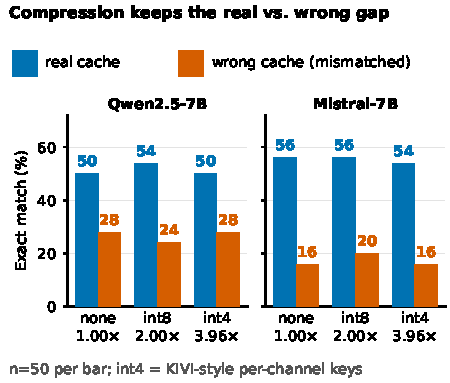
\includegraphics[width=\columnwidth]{figures/fig3_compression.pdf}
\caption{Real versus mismatched (wrong) cache accuracy under compression
(configuration \texttt{A}, $n{=}50$ per bar). Ratios are measured on Qwen2.5 against
the uncompressed 144.35~MB per hop. \textbf{Takeaway: the gap between the real and
the wrong cache survives int8 and KIVI-style int4 on both models, so compression
does not turn the cache into interchangeable state.}}
\label{fig:compression}
\end{figure}


\section{Extended Related Work}
\label{app:relwork}

\paragraph{Rotation-based quantization.}
\label{app:rotation}
We applied a fixed orthonormal
Hadamard rotation to both keys and values before quantizing
(covering PolarQuant's \citep{polarquant2026} rotate-then-quantize
step, not TurboQuant's \citep{turboquant2026} separate QJL
bias-correction term; these are two distinct papers sharing only two
authors, not one work under two names). On our model this produced
severely out-of-distribution decoded output. We traced this to keys'
RoPE encoding: K is cached after RoPE is applied, which mixes channel
pairs by a position-dependent phase, and a second, RoPE-agnostic
rotation disrupts that structure. KIVI \citep{kivi2024} quantizes keys
per-channel and values per-token, motivated by RoPE leaving channel-wise
magnitude more consistent across positions than per-head ranges assume.
RotateKV \citep{rotatekv2025} instead rotates \emph{before} RoPE via
Pre-RoPE Grouped-Head Rotation, explicitly designed to avoid this
interaction. KVQuant \citep{kvquant2024} similarly identifies post-RoPE
key quantization as harder than value quantization for the same reason.

\paragraph{Considered but not adopted compression strategies.}
Orthogonal Backfill \citep{orthobackfill2026} injects a low-rank
residual of discarded content orthogonal to what is retained; its
published formula requires attention weights our \texttt{sdpa} decode
path does not expose, and given our own evidence that naive
reproductions can actively mislead, we did not ship an approximated
version. KVTC \citep{kvtc2026} applies media-compression-style
transform coding (PCA decorrelation, adaptive quantization, entropy
coding) for up to 20x compression, a third paradigm distinct from
uniform quantization and rotation; NVIDIA's kvpress library and
TensorRT-LLM's reuse-aware cache confirm KV compression is an actively
contested axis of deployed systems.

\paragraph{Cheng et al.\ and system-dependence.} Cheng et al.\
\citep{latentcommpay2026} find content-specificity is
\emph{system}-dependent: ceiling effect on LatentMAS, partial on
KVComm, no detected advantage on C2C, holding audit methodology fixed
and varying which published relay system is tested. Our Qwen3-8B
extension independently arrives at the same qualitative pattern while
holding the relay mechanism fixed and varying the model instead. Two
audits converging on ``it depends, and not on accuracy alone'' from
different varied axes is more informative than either alone. ``When KV
Cache Reuse Fails in Multi-Agent Systems'' \citep{kvreusefails2026}
shows reuse strategies effective for generation agents can silently
corrupt an LLM judge's cross-candidate comparison, a complementary
critical-auditing result we do not directly test.

\paragraph{CanonicalMerge.} \citep{canonicalmerge2026} is close to our
fan-in topology: similar-scale models (Qwen3-1.7B/4B versus our
Qwen2.5-7B-Instruct/Mistral-7B-Instruct-v0.3) and a closely related task
(HotpotQA bridge questions versus our full distractor HotpotQA),
addressing a real question we do not (whether merge order biases the
result) but reporting only downstream accuracy, with no
causal-intervention test of whether merged content is specifically, not
just numerously, necessary.

\paragraph{AdaK and Pitfalls of KV Cache Compression.} AdaK
\citep{adak2026} reports adaptive KV-budget estimation generalizing
across Qwen3 (4B/8B) and Mistral-7B-Instruct-v0.2, the same two
architecture families we test, which could look like a counterexample to
our architecture-dependence claim.
We do not believe it is: AdaK estimates budget per-instance and
per-model at inference time rather than committing to one
calibration-time ranking applied uniformly, so it never assumes a
fixed, transferable ranking is safe to act on; its success is a
positive instance of our principle, not a counterexample. This is our
reading of the mechanism, not a reimplementation we verified ourselves.
``The Pitfalls of KV Cache Compression'' \citep{pitfallskv2026} argues
compression methods optimize aggregate metrics while implicitly
equating token retention with functional preservation; our contribution
is a causally grounded, cross-axis demonstration of this within one
system (depth, position, content-identity) rather than the abstract
observation.

\section{Extended Method}
\label{app:method-ext}

\paragraph{Causal-audit baseline caveat.} Zero-ablation is a
known-imperfect causal baseline in the interpretability literature: it
pushes activations off the training distribution, which can produce
large behavioral changes unrelated to whether the zeroed content
carried meaningful information. We treat moment-matched-random and
mismatched, which preserve realistic statistics or substitute another
real cache, as the more informative evidence, and zero-ablation as a
supplementary sanity floor. A fully rigorous ``no difference'' claim
would use a pre-registered equivalence margin rather than absence of
significance; we did not have the budget to pre-register and power such
a test.

\paragraph{Why RLM+KV is implemented from scratch.} We implement the
RLM+KV loop directly on \texttt{transformers} \citep{transformers2020}
rather than \texttt{dspy.RLM}, the first-party DSPy implementation of
RLM. DSPy is built on \texttt{litellm} and is, by design, a text-only,
API-centric orchestration layer: a sub-call through \texttt{dspy.RLM}'s
\texttt{llm\_query} returns decoded text and nothing else, with no
exposure anywhere in the framework to a model's KV cache. Our
\texttt{kv} return channel is not implementable on top of it; we
verified this against DSPy's own documentation before committing to a
from-scratch implementation.

\section{Extended Results}
\label{app:results-ext}

\paragraph{Qualitative texture (sequential chain).} Mismatched's wrong
answers are coherent and grammatical, real linguistic structure
attached to the wrong question; zeroed produces garbled but
recognizable English; random is more degraded still (code-fragment
tokens, mixed-language noise) despite matching real activation
statistics. We read this as a zero vector being a weak attention key
that can be down-weighted, while realistic random noise resembles
genuine signal and actively misdirects attention. A fan-in
garbage-signature scan of all 200 generations gives the identical
texture: 0/50 flagged for real, 4/50 mismatched, 23/50 zeroed, 48/50
random.

\paragraph{Donor-content bleed-through, in full.} Manually reviewing 20
of 36 incorrect \texttt{A\_audit\_mismatched} answers against their
donor question: one unambiguous instance (a Kansas university
fight-song question produced ``Ellie Goulding,'' traceable only to a
donor question about that singer) and one weaker, ambiguous case; the
remainder show ordinary failure on the real question's own topic. One
annotator, no automated classifier or inter-annotator agreement check;
a rigorous version would classify the full set of incorrect examples
automatically or with multiple annotators, which we did not have the
budget to complete.

\paragraph{Layer-selection cost magnitude, full detail.} The
architecture-dependence claim in Section~\ref{sec:results} compares a
near-identical dropped-layer proportion: 9/32 layers (28\%) on Mistral
versus 8/28 layers (29\%) on Qwen2.5. Mistral's cost (30.5 F1 points,
$p=0.0001$) is confirmed significant; Qwen2.5's smaller cost is not yet
significant at $n=100$ ($p=0.34$), but the cross-model claim does not
rest on that reaching significance: even Qwen's most generous
uncertainty bound (F1 CI upper $+16.4$ points) is under half of
Mistral's confirmed collapse. Qwen3-8B's $D$-vs-$A$ comparison ($p=1.0$)
rests on only 3 discordant pairs out of 50, consistent with noise
rather than a real effect.

\paragraph{Mistral layer-selection, full explanation.} On \texttt{C},
mismatched beats zeroed/random ($p=0.0156$ each) but is not
distinguishable from real ($p=0.51$, F1 CI includes zero); \texttt{D}
shows the identical pattern ($p=0.0078$; $p=0.375$). Both track
\texttt{C}/\texttt{D}'s own degraded Mistral baseline (20.0\%/22.0\%
vs.\ Qwen's 46.0\%/50.0\%): less headroom to detect a further
real-vs-mismatched gap on an already-degraded baseline, not a failure
to replicate content-dependence. \texttt{B\_int8} on Mistral replicates
the full clean pattern, matching every quantization-only configuration;
layer-selection configurations show the attenuated pattern,
quantization-only configurations do not, consistently across two
separate experiments.

\paragraph{GSM8K confirmatory run.} $n=50$, Qwen2.5: \texttt{D} matched
\texttt{A}'s accuracy exactly (McNemar $p=1.0$, more decisively free
than on HotpotQA); the causal audit's three-tier ordering held with
every comparison significant ($p<0.0002$), larger effect sizes than the
original HotpotQA run. One run on one additional task, not a systematic
multi-task study; we did not extend \texttt{B\_int8}/\texttt{D}-family
audits or Mistral to GSM8K.

\paragraph{2WikiMultihopQA confirmatory run, verification detail.}
\label{app:2wiki}
All four conditions (\texttt{A} and its three audit variants) were
scored on the identical 50 paired examples, confirmed by matching
example index, question text, and gold answer across conditions. The
mismatched condition drew from a held-out donor pool of 20 distinct
questions; checking every donor question against all 50 scored
questions directly, none matched, and all 100 mismatched substitutions
(50 examples times two relay hops) were confirmed applied via the
per-example audit logs. Accuracy, F1, and latency were independently
reconstructed from the per-example records and matched the evaluator's
own summary exactly. Real versus mismatched had 19 discordant pairs,
all 19 favoring real and none favoring mismatched, F1 delta $+39.1$
points, 95\% bootstrap CI $[+26.1, +52.3]$. This is a single
confirmatory run on one additional dataset and one configuration, not a
systematic cross-dataset study.

\paragraph{Fan-in mismatched-vs-zeroed/random leg.} Not significant by
exact McNemar ($p=0.25$ each, 3 discordant pairs, the test's own floor
at that count), but the F1 bootstrap CI excludes zero for both
($+0.112$ [$+0.035,+0.200$], $+0.120$ [$+0.047,+0.206$]):
accuracy-level evidence is underpowered at this $n$ for this specific
leg while the finer-grained F1 comparison trends real.

\section{Qwen3-8B Verification}
\label{app:qwen3}

We verified the Qwen3-8B exception (Section~\ref{sec:results}) is a
real effect, not a bug, three ways: no donor-question pool leakage;
\texttt{A\_audit\_zeroed} and \texttt{D\_audit\_zeroed} produce
byte-identical output on all 50 examples, which looked alarming until
traced to \texttt{D}'s own \texttt{zeros} reconstruction strategy
composing correctly with the audit's own zeroing, not a bug; and real,
zeroed, and mismatched overlap on only 10--24 of 50 examples pairwise,
confirming the substitution takes effect selectively rather than being
silently inert. We do not have a mechanistic explanation for the
difference; we report it as an empirical observation and flag candidate
mechanisms as future work.

\section{RLM+KV Behavioral Signal}
\label{app:behavioral}

Timeout rate, mean turn count, and mean delegation-call count are
monotonic across conditions (real 22\% timeout, 7.72 turns, 1.38 calls;
mismatched 42\%/8.48/1.12; zeroed 72\%/9.46/0.76; random 76\%/9.60/0.66).
Substituting ``session finished without exhausting its turn budget''
for ``correct'' in the same paired McNemar test, every comparison is
significant, including mismatched versus random ($p<0.0001$), exactly
the leg final-answer accuracy left unresolved (real vs.\ mismatched
$p=0.0309$; real vs.\ zeroed/random $p<0.0001$ each; mismatched vs.\
zeroed $p=0.0001$). We verified this run shows no new degenerate output
at this scale (0/50 flagged for real/text; a clean, monotonic
3/50--48/50 ordering across the remaining conditions).

\section{RLM+KV Non-Determinism: Diagnosis and Fix}
\label{app:nondeterminism}

An earlier run of this experiment was not run-to-run deterministic.
Diffing raw generations for the identical 50 questions between two
independent runs under greedy decoding found 15 of 50 (30\%)
\texttt{text}-channel examples produced genuinely different output,
plausibly GPU floating-point non-associativity cascading through this
prototype's long, self-referential decode loop (unlike the two fixed
topologies, confirmed bit-identical across reruns). We fixed this by
forcing \texttt{torch.use\_deterministic\_algorithms(True,
warn\_only=True)} and setting \texttt{CUBLAS\_WORKSPACE\_CONFIG} before
any CUDA context exists. Verification: a rerun of the \texttt{text}
channel on 20 questions produced 0/20 differing raw answers against the
pre-fix run, including all 7 of the originally divergent examples. We
then reran the full five-channel, $n=50$ ladder and diffed every field,
not only the ones reported in Section~\ref{sec:results}: exact match,
F1, timeout rate, and delegation-call count are bit-identical across
both runs (0 of 250 raw answers differ). One harmless nuance: 33 of the
\texttt{random} condition's 50 examples show different intermediate
turn-by-turn wording despite both independently exhausting their turn
budget on the identical question with the identical final outcome; this
never affects any scored quantity in this paper.

Separately, getting a working baseline for this topology at all
required diagnosing and fixing three real engineering failure modes: a
sub-call's own prompt framing leaking into the receiver's attention
when spliced without isolating the generated answer span; a
session-wide repetition-tracking loss specific to a persistent,
turn-continuing cache; and a RoPE position-shift bug specific to
splicing an answer-only, prompt-truncated child KV, verified two ways
(a corrected unit test and a real-model rerun showing every previously
degenerate example become coherent).

\section{Fan-in Causal Audit: Design Bug and Fix}
\label{app:faninbug}

An early version substituted only one of two children's KV by default,
leaving the other's real content as an unaudited shortcut. This
produced a near-null pilot result (3/10 exact-match for real versus
3/10 for zeroed) that, on inspection, was a weaker test than intended:
5 of 10 zeroed-condition outputs already showed the expected
garbled-output signature, meaning the aggregator was still succeeding
on the uncorrupted child often enough to mask the effect. We fixed this
by substituting every child's KV (extracted into a directly testable
helper function with its own unit tests), matching the full-relay-
corruption strength of the sequential pipeline's own audit. The
corrected result is the one reported in Section~\ref{sec:results}.

\section{Nibble-Packing: Byte-Accounting Bug and Real Fix}
\label{app:nibble}

Our compressor initially stored every quantized tensor as one full
\texttt{torch.uint8} per element regardless of bit-width, so a 4-bit
value took the same byte an 8-bit value did; first-reported compression
ratios assumed packing that did not exist. We implemented genuine
two-values-per-byte packing (pack after quantizing for \texttt{bits==4},
unpack before dequantizing), verified via unit tests covering
round-trip exactness (including odd-length/padding edge cases,
full-nibble-range coverage) and, most directly, bit-identical
\texttt{compress}/\texttt{decompress} output with and without packing,
confirming packing is a pure storage-format change. The corrected
ratios land back at almost exactly the originally reported figures: the
original formula's arithmetic (0.5 bytes/element for 4-bit) was always
what real packing would produce; the bug was that nothing in the
compressor actually packed anything. This is unit-tested at the tensor
level, not confirmed via a live GPU rerun of the full pipeline with
packing enabled; reported accuracy/F1 figures come from pre-packing
runs, only compression-ratio figures reflect the packing-enabled
compressor.

\section{Layer-Selection Failure Character: Full Statistics}
\label{app:failurechar}

Qwen's incorrect \texttt{D} answers average 18 characters, 2\%
exceeding 150, overwhelmingly close near-misses (reformatted dates,
dropped honorifics, single-character typos). Mistral's average 109
characters, 15\% exceeding 150, maximum 1,454, including fluent
fabricated tangents (e.g.\ a full invented biography of an unrelated
person) and degenerate repetition loops essentially absent from Qwen's
failure set. We checked the obvious confound, that our fixed
repetition penalty under-penalizes Mistral relative to its own tuned
defaults, against each model's published \texttt{generation\_config.json}:
Qwen's own default is exactly our setting (1.05); Mistral's specifies
none, so our setting applies \emph{more} correction for Mistral, the
opposite of what the confound needs. The long-tail pattern persists
anyway.

\section{Additional Configurations and Tables}
\label{app:extratables}

\begin{table}[h]
\centering
\small
\caption{Compression on the uncompressed-relay chain, Qwen2.5-7B-Instruct,
HotpotQA, $n{=}100$. Ratios are relative to \texttt{A}'s 144.35~MB per hop;
latency and no-relay baselines are in Table~\ref{tab:full}.}
\label{tab:main}
\begin{tabular}{lcc}
\toprule
\textbf{Config} & \textbf{Acc.\ / F1} & \textbf{KV/hop} \\
\midrule
A & 56.0 / 69.1 & 144.35 MB \\
B\_int8 & 57.0 / 70.5 & 72.16 MB (2.00x) \\
B\_int4 & 0.0 / 0.0 & 38.38 MB (4.00x) \\
\textbf{B\_int4\_kivi} & \textbf{52.0 / 64.1} & 36.43 MB (3.96x) \\
C & 43.0 / 57.8 & 104.16 MB \\
D & 50.0 / 61.9 & 37.82 MB (3.82x) \\
E & 9.0 / 17.4 & 35.63 MB \\
\bottomrule
\end{tabular}
\end{table}

Table~\ref{tab:full} reports every configuration's latency alongside
accuracy/F1/KV-per-hop, the full version of Table~\ref{tab:main}
including the two no-relay controls and \texttt{E\_int8}. We report
compressed bytes and latency as two distinct quantities throughout this
paper (Section~\ref{sec:results}): our evaluation has no network
transmission, and a smaller cache does not measurably speed up our
single-GPU pipeline.

\begin{table}[h]
\centering
\small
\begin{tabular}{lcccc}
\toprule
\textbf{Config} & \textbf{Acc.} & \textbf{F1} & \textbf{Lat.} & \textbf{KV/hop} \\
\midrule
single\_agent & 57.0 & 68.4 & 1.6s & --- \\
text\_agent & 54.0 & 68.3 & 7.2s & --- \\
A & 56.0 & 69.1 & 8.6s & 144.35 MB \\
B\_int8 & 57.0 & 70.5 & 8.3s & 72.16 MB \\
B\_int4 & 0.0 & 0.0 & 39.4s & 38.38 MB \\
B\_int4\_kivi & 52.0 & 64.1 & 9.6s & 36.43 MB \\
C & 43.0 & 57.8 & 10.0s & 104.16 MB \\
D & 50.0 & 61.9 & 10.2s & 37.82 MB \\
E & 9.0 & 17.4 & 19.8s & 35.63 MB \\
E\_int8 & 1.0 & 6.2 & 22.2s & 49.05 MB \\
\bottomrule
\end{tabular}
\caption{Full version of Table~\ref{tab:main} (Qwen2.5-7B-Instruct,
HotpotQA, $n=100$), with latency and the no-relay controls.}
\label{tab:full}
\end{table}

\texttt{single\_agent} and \texttt{text\_agent} are no-KV-relay
controls: every KV-relay configuration shares identical prompts with
\texttt{text\_agent}, so accuracy/latency deltas are attributable to
the relay mechanism itself. \texttt{E\_int8} (uniform-int8 variant of
the offset-correction baseline) also fails catastrophically, like the
offset-correction baseline \texttt{E} (9.0/17.4 in Table~\ref{tab:main}); we do not
use either in the audit. Fixing KIVI's value side
too (\texttt{B\_int4\_kivi\_full}, per-token quantization) does not
improve on \texttt{B\_int4\_kivi} (44.0\% vs.\ 50.0\% on a matched
50-example subset, $p=0.51$, trending the other way) and is worse on
compression (3.75x vs.\ 3.99x self-referential): per-token quantization
stores a scale/zero-point pair per sequence position, and sequence
length vastly exceeds K's per-channel grouping (128 channels). Together
with an earlier null result for rotating values instead, two
independently motivated value-side interventions both failed, evidence
the key/RoPE interaction was \texttt{B\_int4}'s entire failure
mechanism, not one of several factors.

\section{Scope and Engineering Detail}
\label{app:limitations}

\paragraph{Single-process, single-GPU.} Every experiment runs within
one Python process on one RTX 4090; compression-ratio and
transmitted-byte accounting reflects what a real distributed deployment
would need to send, but latency numbers exclude network transfer, and
smaller relayed caches are not observed to be faster, since the model
executes every transformer layer regardless of injected-cache contents.
A systems-scale deployment study (multi-GPU, real network transfer,
concurrent load) was out of scope.

\paragraph{Scope detail.} A fourth model family, Phi-3.5-mini-instruct, was dropped after a pre-existing LongRoPE limitation unrelated to our pipeline: plain \texttt{model.generate()} degrades past its 4{,}096-token original context, which HotpotQA's cumulative relay contexts routinely exceed. All of our architecture variation is between pipeline runs, not within one pipeline mixing architectures across agent roles. A genuinely adversarial fan-in \citep{latentagentslie2026} and LatentMAS's layer-wise KV concatenation \citep{latentmas2026} remain untested against our methodology, and all results use greedy decoding.

\paragraph{Partial reproduction.} Our rotation-based quantization omits
TurboQuant's QJL bias-correction term; our KIVI-inspired fix omits the
original method's group-wise windowing and fp16 residual buffer. Both
are inspired-by implementations scoped to test a specific hypothesis,
not certified reproductions.

\end{document}
